% Drawing 154/08-8 -- folder 154, batch 08, archive page 152 (PDF page 153).
% Transcription: en haut, deux dessins de fuseaux : l'un au crayon, traversé de pseudo-droites, avec deux flèches noires d'un bord à l'autre ; l'autre en couleur, bordé d'orange, rempli de courbes vertes et de tirets bruns qui joignent les deux pointes, traversé d'un réseau de droites brunes qui se croisent en losanges, avec de petites flèches aux croisements
% Kind: pencil spindle with two arrows; coloured spindle with green curves, brown dashes and a lozenge net of brown lines. Method 2 (schematic redraw from the facsimile). Status: partial.
% Notes: At the top of the (portrait) sheet, two drawings of spindles: one in pencil, crossed by pseudolines, with two black arrows from one edge to the other; the other in colour, bordered in orange, filled with green curves and brown dashes joining the two tips, crossed by a net of brown lines crossing in lozenges, with small arrows at the crossings (left out). The zigzag spindle lower on the page is not covered by this mark. Read from the page view; the net is regularised. Still differs from the facsimile: At the top of the (portrait) sheet, two drawings of spindles: one in pencil, crossed by pseudolines, with two black arrows from one edge to the other; the other in colour, bordered in orange, filled with green curves and brown dashes joining the two tips, crossed by a net of brown lines crossing in lozenges, with small arrows at the crossings (left out). The zigzag spindle lower on the page is not covered by this mark.
% Coordinates: 1 unit = 1 mm = 1/100 of the crop width (bbox in page fractions: [0.242, 0.12, 0.73, 0.363]).
% Redrawn by Claude (claude-opus-5-5), issue #73, 2026-11-07; not checked by a human; not compiled (no TeX in the session).
% Revised by Claude (claude-opus-5-5) 2026-11-09 (issue #128) after Michel's check: vertices snapped to exact intersections (drawn points on their lines, meeting ends on the stroke they meet, near-concurrent lines through one computed point, curve ends on their rim); labels at \small as in folder 80 batch 3. Status: partial.
% Rights: reproduces part of the work -- behind RENDER_TRANSCRIPTS, never published by itself.
\documentclass[tikz,border=3pt]{standalone}
\usepackage{amsmath,amssymb}
\usetikzlibrary{patterns,arrows.meta}
\tikzset{Or/.style={orange!90!black}, Ye/.style={yellow!80!orange}, Lg/.style={green!60!black!70}, Dg/.style={green!45!black}, Br/.style={brown!80!black}, Rd/.style={red!85!black}, Bl/.style={blue!70!black}, Gy/.style={black!40}, pencil/.style={black!45}, struck/.style={black!35}, mark/.style={circle,draw,inner sep=1.3pt}, pt/.style={circle,fill,inner sep=0.9pt}, opt/.style={circle,draw,fill=white,inner sep=1.1pt}}
\begin{document}
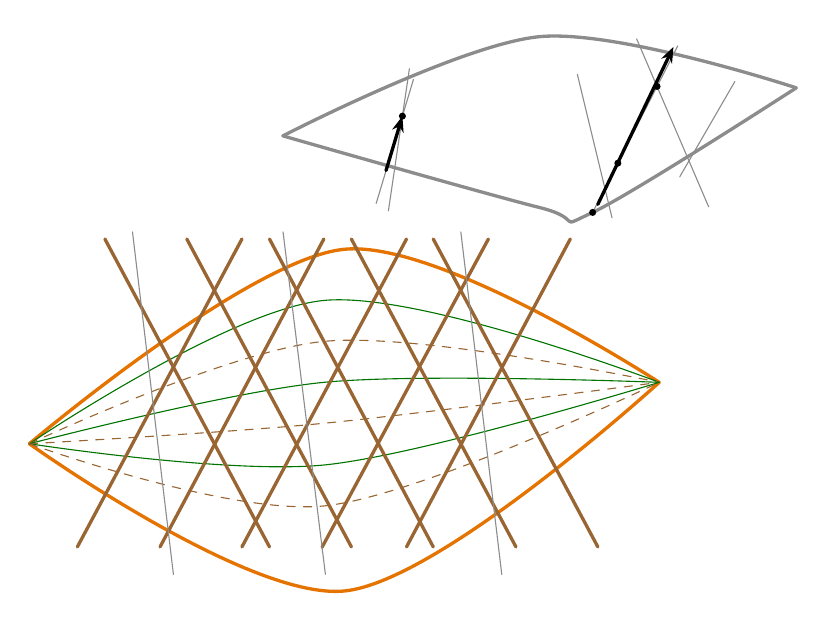
\begin{tikzpicture}[x=1mm,y=1mm,line cap=round,line join=round,font=\scriptsize]
\draw[pencil,very thick] plot[smooth, tension=0.55] coordinates {(33.9,-13.9) (66.5,-1.3) (99.1,-7.8)};
\draw[pencil,very thick] plot[smooth, tension=0.55] coordinates {(33.9,-13.9) (66.5,-23) (73.24,-23.62) (99.1,-7.8)};
\draw[pencil] (45.75,-22.48) -- (50.48,-6.73);
\draw[pencil] (49.97,-5.37) -- (47.3,-23.43);
\draw[pencil] (73.24,-23.62) -- (84.05,-2.48);
\draw[pencil] (71.3,-6.1) -- (75.7,-24.3);
\draw[pencil] (78.83,-1.59) -- (87.97,-22.9);
\draw[pencil] (91.3,-7) -- (84.3,-19.1);
\draw[-{Stealth[length=2mm]},very thick] (47,-18.3) -- (49.08,-11.39);
\draw[-{Stealth[length=2mm]},very thick] (73.9,-22.6) -- (83.5,-2.6);
\node[pt] at (49.08,-11.39) {};
\node[pt] at (76.44,-17.37) {};
\node[pt] at (81.42,-7.62) {};
\node[pt] at (73.24,-23.62) {};
\draw[Or,very thick] plot[smooth, tension=0.55] coordinates {(1.7,-53) (41.7,-28.3) (81.7,-45.2)};
\draw[Or,very thick] plot[smooth, tension=0.55] coordinates {(1.7,-53) (41.7,-71.7) (81.7,-45.2)};
\draw[Dg] plot[smooth, tension=0.55] coordinates {(1.7,-53) (39.1,-34.8) (81.7,-45.2)};
\draw[Br,dashed] plot[smooth, tension=0.55] coordinates {(1.7,-53) (39.1,-40) (81.7,-45.2)};
\draw[Dg] plot[smooth, tension=0.55] coordinates {(1.7,-53) (39.1,-45.2) (81.7,-45.2)};
\draw[Br,dashed] plot[smooth, tension=0.55] coordinates {(1.7,-53) (39.1,-50.4) (81.7,-45.2)};
\draw[Dg] plot[smooth, tension=0.55] coordinates {(1.7,-53) (39.1,-55.7) (81.7,-45.2)};
\draw[Br,dashed] plot[smooth, tension=0.55] coordinates {(1.7,-53) (39.1,-60.9) (81.7,-45.2)};
\draw[Br,very thick] (7.8,-66.1) -- (28.7,-27);
\draw[Br,very thick] (18.3,-66.1) -- (39.1,-27);
\draw[Br,very thick] (28.7,-66.1) -- (49.6,-27);
\draw[Br,very thick] (38.88,-66.13) -- (60,-27);
\draw[Br,very thick] (49.6,-66.1) -- (70.4,-27);
\draw[Br,very thick] (11.3,-27) -- (32.2,-66.1);
\draw[Br,very thick] (21.7,-27) -- (42.6,-66.1);
\draw[Br,very thick] (32.2,-27) -- (53,-66.1);
\draw[Br,very thick] (42.6,-27) -- (63.5,-66.1);
\draw[Br,very thick] (53,-27) -- (73.9,-66.1);
\draw[pencil] (14.8,-26.1) -- (20,-69.6);
\draw[pencil] (33.92,-26.1) -- (39.3,-69.58);
\draw[pencil] (56.5,-26.1) -- (61.7,-69.6);
\end{tikzpicture}
\end{document}
